
\chapter[Dạng bài: Sóng cơ và các đặc trưng của sóng cơ]{Dạng bài: Sóng cơ và các đặc trưng của sóng cơ}
\section{Lý thuyết}
\subsection{Định nghĩa}

Sóng cơ là dao động cơ lan truyền trong môi trường.
\luuy{Khi sóng cơ truyền đi chỉ có \bltext{pha dao động} của các phần tử vật chất lan truyền còn các phần tử vật chất thì không truyền đi mà chỉ dao động xung quanh \bltext{vị trí cân bằng} cố định.}
\subsection{Phân loại}
Sóng cơ chia làm 2 loại: sóng ngang và sóng dọc.
\begin{itemize}
	\item Sóng ngang là sóng trong đó các phần tử của môi trường dao động theo phương \bltext{vuông góc} với phương truyền sóng. Sóng ngang truyền được trong \bltext{chất rắn}, trên \bltext{bề mặt chất lỏng}.
	\item Sóng dọc là sóng trong đó các phần tử của môi trường dao động theo phương \bltext{trùng} với phương truyền sóng. Sóng dọc truyền được trong môi trường \bltext{rắn}, \bltext{lỏng}, \bltext{khí}.
\end{itemize}
\begin{center}
	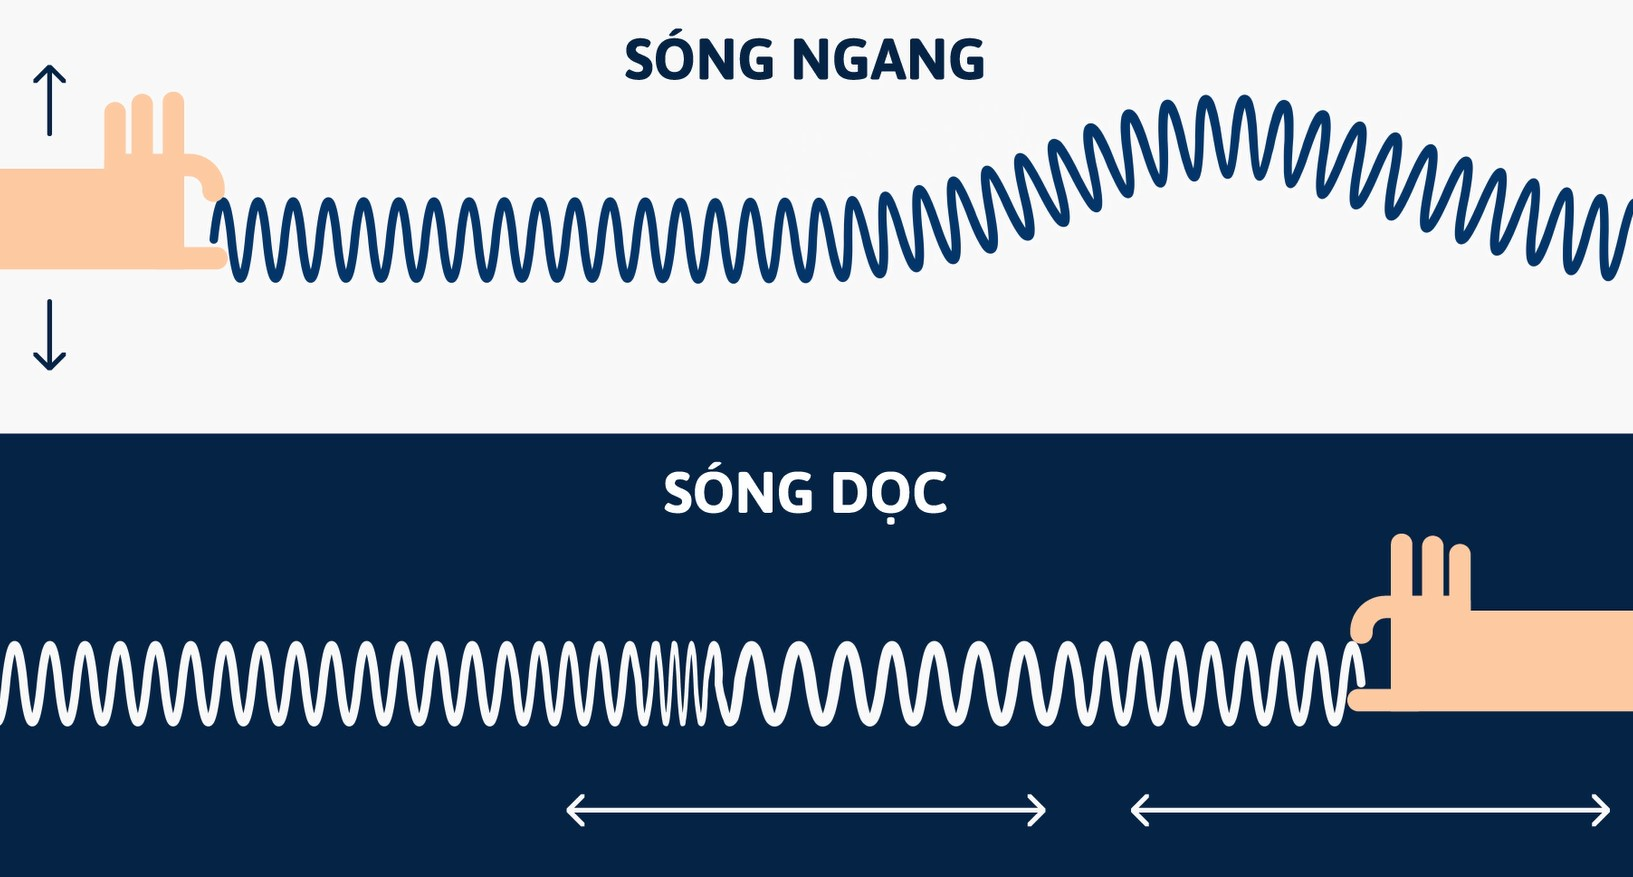
\includegraphics[scale=0.3]{../figs/VN12-PH-10-L-005-1-V2-1.jpg}
\end{center}
\subsection{Các đặc trưng của một sóng hình sin}

\begin{tabular}{|m{8cm}|m{4cm}|}
	\hline
	\thead{Định nghĩa}	& \thead{Ký hiệu, công thức} \\
	\hline
	Biên độ dao động của sóng là biên độ dao động của một phân tử của môi trường có sóng truyền qua. & \[A\]  \\
	\hline
	Chu kỳ của sóng là chu kỳ dao động của một phần tử của môi trường có sóng truyền qua. & \[T\] \\
	\hline
	Tần số của sóng là nghịch đảo của chu kỳ sóng. & \[f=\dfrac{1}{T}\]   \\
	\hline	
	Tốc độ truyền sóng là tốc độ lan truyền dao động trong môi trường.	&\[v\]    \\
	\hline
	Bước sóng là quãng đường mà sóng truyền được trong một chu kỳ. & \[\lambda = vT=\dfrac{v}{f}\]\\
	\hline
	Năng lượng sóng là năng lượng dao động của các phần tử của môi trường có sóng truyền qua. &  \[W\]  \\
	\hline
\end{tabular}

\subsection{Hình dạng sóng}

\begin{itemize}
	\item Khoảng cách giữa $n$ gợn sóng liên tiếp $d$:
	\begin{equation*}
		d=(n-1)\lambda \Rightarrow \lambda = \dfrac{d}{n-1}.
	\end{equation*}
	\item Khoảng cách từ gợn $n$ đến gợn thứ $m$ ($m>n$) $d$:
	\begin{equation*}
		d=(m-n)\lambda \Rightarrow \lambda = \dfrac{d}{n+m-n}.
	\end{equation*}
	\item Nhô cao lên $N$ lần trong thời gian $\Delta t$:
	\begin{equation*}
		\Delta t = (N-1)T \Rightarrow T =\dfrac{\Delta t}{N-1}.
	\end{equation*}
\end{itemize}
\begin{center}
	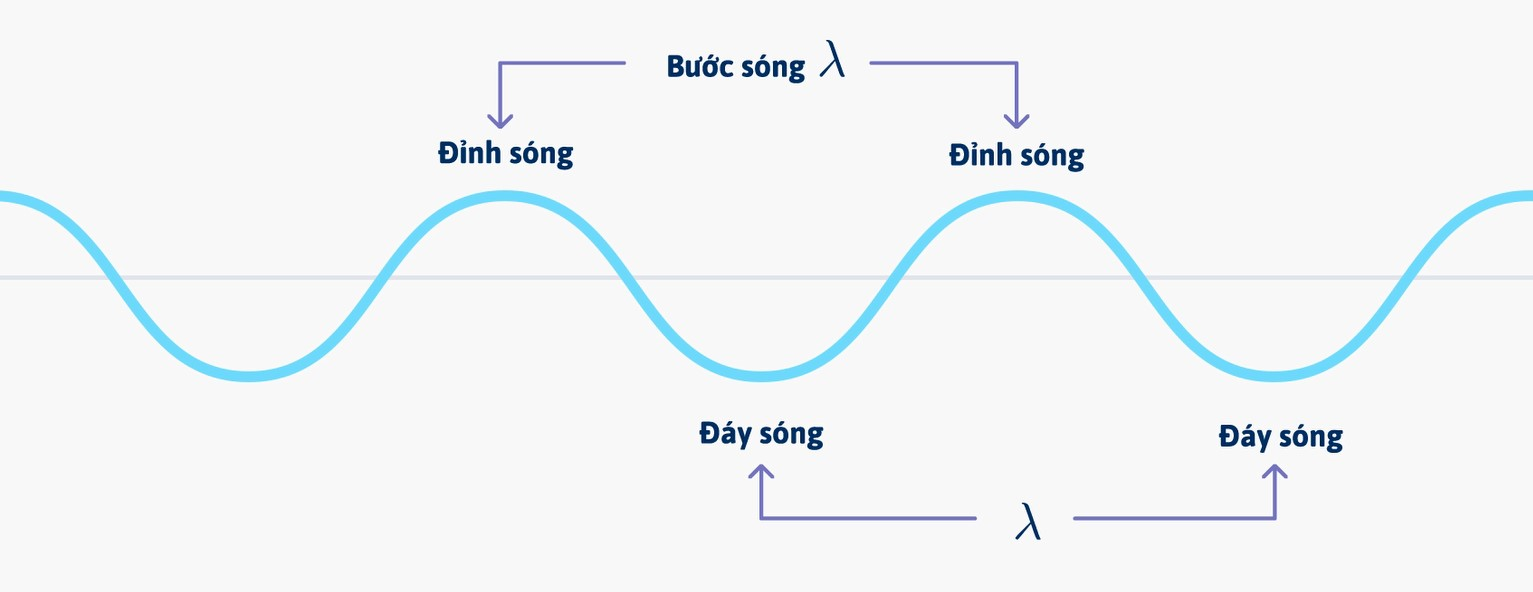
\includegraphics[scale=0.4]{../figs/VN12-PH-10-L-005-1-V2-2.jpg}
\end{center}
\section{Mục tiêu bài học - Ví dụ minh họa}
\begin{dang}{Ghi nhớ được định nghĩa\\ sóng cơ, sóng ngang, sóng dọc}
	\viduii{1}{Sóng cơ là
		\begin{mcq}
			\item sự truyền chuyển động cơ trong không khí.
			\item những dao động cơ lan truyền trong môi trường.
			\item chuyển động tương đối của vật này so với vật khác.
			\item sự co dãn tuần hoàn giữa các phần tử của môi trường.
		\end{mcq}
	}
	{
		\begin{center}
			\textbf{Hướng dẫn giải}
		\end{center}
		
		Sóng cơ là những dao động cơ lan truyền trong môi trường.
		
		
		\textbf{Đáp án: B}.
	}
	
	\viduii{1}
	{
		Khi nói về sóng cơ, phát biểu nào dưới đây là \textbf{sai}?
		\begin{mcq}
			\item Sóng dọc là sóng mà phương dao động của các phần tử vật chất nơi sóng truyền qua trùng với phương truyền sóng.
			\item Sóng cơ không truyền được trong chân không.
			\item Sóng ngang là sóng mà phương dao động của các phần tử vật chất nơi sóng truyền qua vuông góc với phương truyền sóng.
			\item Khi sóng truyền đi, các phần tử vật chất nơi sóng truyền qua cùng truyền đi theo sóng.
		\end{mcq}
	}{
		\begin{center}
			\textbf{Hướng dẫn giải}
		\end{center}
		
		Khi sóng cơ truyền đi chỉ có \bltext{pha dao động} của các phần tử vật chất lan truyền còn các phần tử vật chất thì không truyền đi mà chỉ dao động xung quanh \bltext{vị trí cân bằng} cố định.
		
		\textbf{Đáp án: D.}
	}
	
\end{dang}
\begin{dang}{Ghi nhớ được các đặc trưng của sóng cơ}
	\viduii{1}{Bước sóng là
		\begin{mcq}
			\item quãng đường mà mỗi phần tử của môi trường đi được trong 1 giây.
			\item khoảng cách giữa hai phần tử của sóng dao động ngược pha.
			\item khoảng cách giữa hai phần tử sóng gần nhau nhất trên phương truyền sóng dao động cùng pha.
			\item khoảng cách giữa hai vị trí xa nhau nhất của mỗi phần tử sóng.
		\end{mcq}
	}
	{
		\begin{center}
			\textbf{Hướng dẫn giải}
		\end{center}
		
		Định nghĩa 1: Bước sóng là khoảng cách giữa hai phần tử sóng gần nhau nhất trên phương truyền sóng dao động cùng pha.
		
		Định nghĩa 2: Bước sóng là quãng đường mà sóng truyền được trong một chu kỳ.
		
		
		\textbf{Đáp án: C}.
	}
	
	\viduii{2}
	{
		Khi sóng cơ truyền càng xa nguồn thì 
		\begin{mcq}
			\item biên độ sóng càng giảm.
			\item tần số sóng càng giảm.
			\item bước sóng càng giảm.
			\item biên độ và năng lượng sóng càng giảm.
		\end{mcq}
	}{
		\begin{center}
			\textbf{Hướng dẫn giải}
		\end{center}
		
		Khi sóng cơ truyền càng xa nguồn thì biên độ và năng lượng sóng càng giảm.
		
		\textbf{Đáp án: D.}
	}
	
\end{dang}
\begin{dang}{Sử dụng được các công thức tính tốc độ truyền sóng, bước sóng, tần số}
	\viduii{3}{Một người quan sát một chiếc phao trên mặt biển, thấy nó nhô cao $10$ lần trong khoảng thời gian $\SI{36}{\second}$ và đo được khoảng cách giữa 3 đỉnh sóng liên tiếp là $\SI{36}{\meter}$. Tốc độ truyền sóng là
		\begin{mcq}(4)
			\item $\SI{2.8}{\meter/\second}$.
			\item $\SI{3.6}{\meter/\second}$.
			\item $\SI{1.7}{\meter/\second}$.
			\item $\SI{4.5}{\meter/\second}$.
		\end{mcq}
	}
	{
		\begin{center}
			\textbf{Hướng dẫn giải}
		\end{center}
		
		Thời gian giữa 10 lần chiếc phao nhô cao ứng với 9 chu kì nên ta tính được thời gian của một chu kỳ như sau:
		$$\Delta t=9T=\SI{36}{s}\Rightarrow T=\SI{4}{\second}.$$
		
		Khoảng cách giữa 3 đỉnh sóng liên tiếp là 2 bước sóng nên ta tính được bước sóng như sau:
		$$\Delta d=2\lambda=\SI{36}{m}\Rightarrow \lambda=\SI{18}{\meter}.$$
		
		Tốc độ truyền sóng của sóng này là:
		$$v=\dfrac{\lambda}{T}=\dfrac{\SI{18}{\meter}}{\SI{4}{\second}}=\SI{4.5}{\meter/\second}.$$
		
		
		\textbf{Đáp án: D}.
	}
	
	\viduii{3}
	{
		Khoảng cách giữa 15 đỉnh sóng liên tiếp là $\SI{3,5}{m}$. Thời gian truyền sóng trên khoảng cách đó là $\SI{7}{s}$. Tính tần số, bước sóng và tốc độ truyền của sóng.
	}{
		\begin{center}
			\textbf{Hướng dẫn giải}
		\end{center}
		
		Ta có khoảng cách 15 đỉnh sóng liên tiếp là $\SI{3,5}{m}$:
		\begin{equation*}
			14\lambda = \SI{3,5}{m} \Rightarrow \lambda = \SI{0,25}{m}.
		\end{equation*}
		
		Vận tốc của sóng:
		\begin{equation*}
			v=\dfrac{s}{t} = \SI{0,5}{s}.
		\end{equation*}
		
		Tần số của sóng:
		\begin{equation*}
			f = \dfrac{v}{\lambda} =\SI{2}{Hz}.
		\end{equation*}
		
	}
	
\end{dang}